\documentclass[10pt]{article}
\usepackage[latin1]{inputenc}
\usepackage{amsmath}
\usepackage{amsfonts}
\usepackage{amssymb}
\usepackage{graphicx}
\begin{document}
	
	\title{MATH 387 Midterm Part I. Theory}
	\author{Niklas Brake, 260602499}
	\maketitle
	
	\paragraph{(a)}
	Let $$\tilde{D}_h=\frac{f(h)+\delta f(h)-f(-h)-\delta f(-h)}{2h} $$
	Then, $$\tilde{D}_h=\frac{f(h)-f(-h)}{2h} + \frac{\delta f(h)-\delta f(-h)}{2h}$$
	By Taylor's Theorem and the Mean Value Theorem, $\exists \xi_1 \in (0,h)$ and $\xi_2 \in (-h,0)$ such that
	\begin{align*}
	f(h)&=f(0)+hf'(0)+\frac{h^2}{2}f''(0)+\frac{h^3}{6}f'''(\xi_1) \\
	f(-h)&=f(0)-hf'(0)+\frac{(-h)^2}{2}f''(0)+\frac{(-h)^3}{6}f'''(\xi_2)
	\end{align*}
	Thus,
	$$f(h)-f(-h) = 2hf'(0)+\frac{h^3}{6}\left(f'''(\xi_1)+f'''(\xi_2)\right) $$
	Now since $f'''$ is continuous, by the Intermediate Value Theorem, $\exists \xi \in (-h,h)$ such that $f'''(\xi)=\frac{f'''(\xi_1)+f'''(\xi_2)}{2}$. Therefore,
	\begin{align*}
	&f(h)-f(-h) = 2hf'(0)+\frac{h^3}{3}f'''(\xi) \\
	&\Rightarrow \tilde{D}_h=f'(0)+\frac{h^2}{6}f'''(\xi) + \frac{\delta f(h)-\delta f(-h)}{2h} \\
	&\Leftrightarrow \tilde{D}_h-f'(0)=\frac{h^2}{6}f'''(\xi) + \frac{\delta f(h)-\delta f(-h)}{2h}
	\end{align*}
	
	\paragraph{(b)}
	Since $h\in (-a,a)$, $\left| \delta f(h)\right| <\varepsilon$. Further, since $f'''$ is continuous on a closed interval, it is bounded by some constant $M<\infty$.
	\begin{align*}
	 \left|\tilde{D}_h-f'(0)\right|  &= \left|\frac{h^2}{6}f'''(\xi) + \frac{\delta f(h)-\delta f(-h)}{2h} \right| \\
	   & \le \left|\frac{h^2}{6}f'''(\xi)\right| + \left|\frac{\delta f(h)-\delta f(-h)}{2h}\right|  \\
	    &\le \frac{h^2}{6} \max_{x\in[-a,a]} \left|f'''(x)\right| + 2\left|\frac{\delta f(h)}{2h}\right| \\
	     &\le \frac{h^2}{6}M+\frac{\varepsilon}{h} 
     \end{align*}
     
     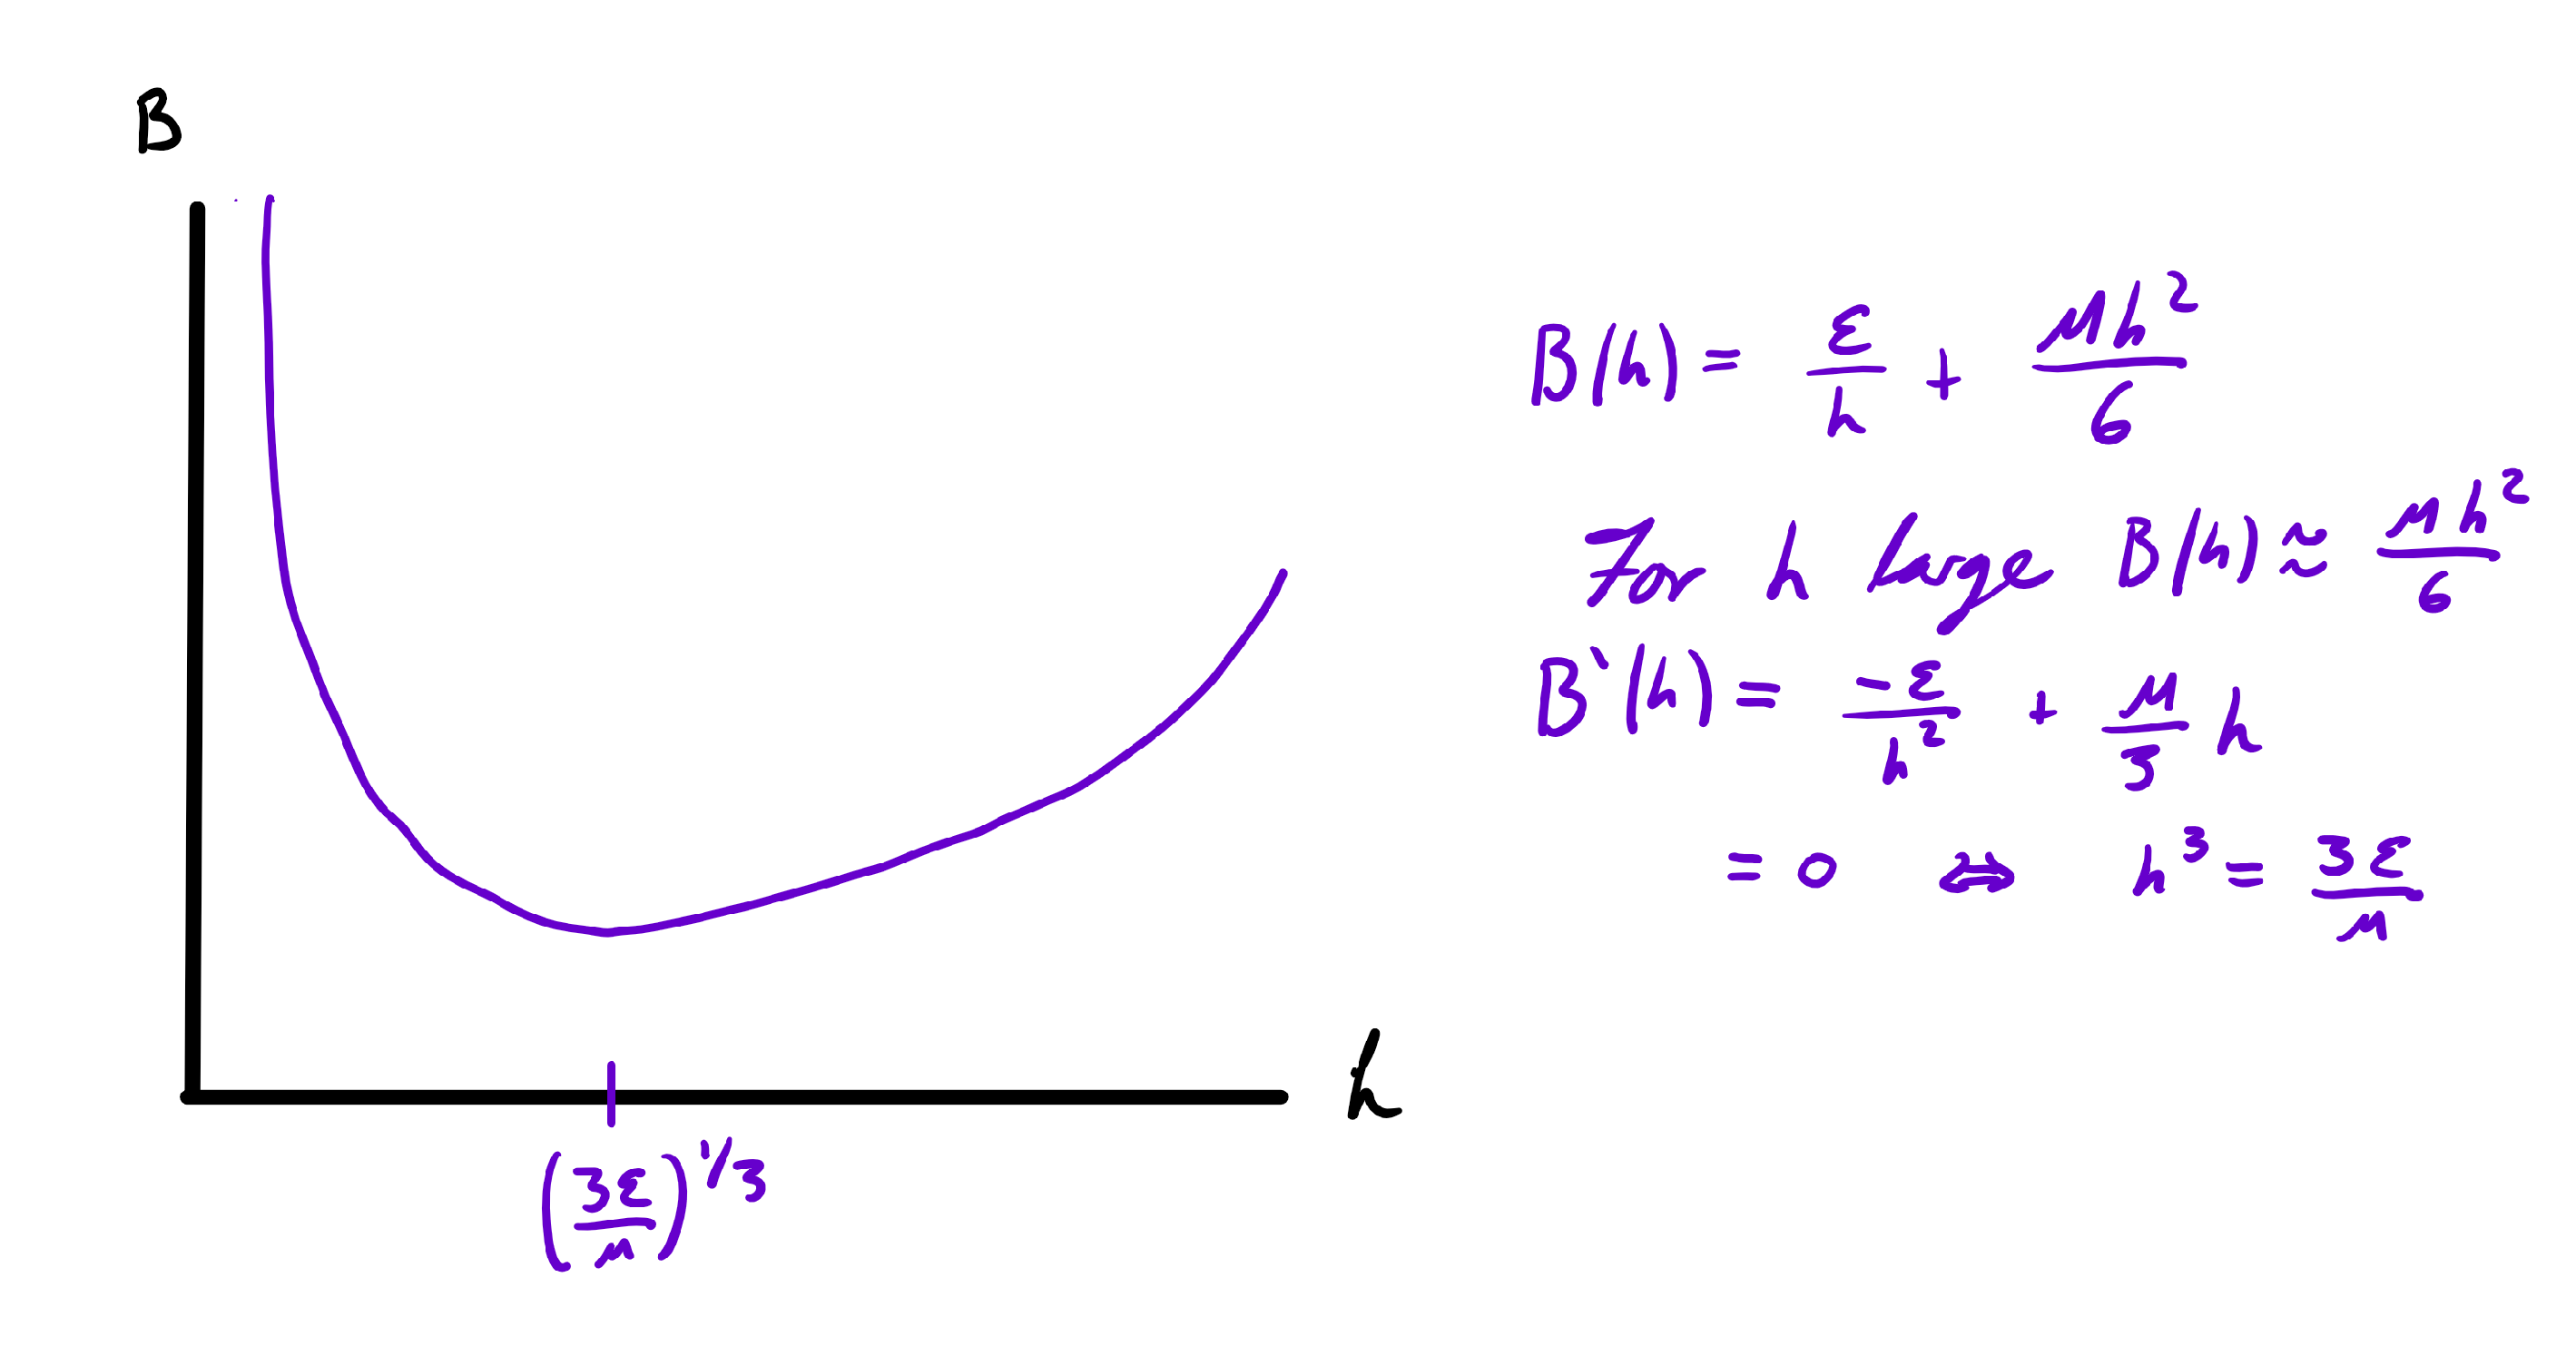
\includegraphics[width=\linewidth]{Sketch.png}
     
     Since $B\to\infty$ as $h\to0$, if we take $h$ to be too small, we cannot bound our error. Thus, we should take $h$ such that we can bound our error as small as possible. This occurs when $B'(h)=0$, which gives us $h=\left(\frac{3\varepsilon}{M}\right)^{1/3}$
     
\end{document}